% Traductions et équivalences

\begin{frame}[c]
  \frametitle{Équivalences entre les sémantiques de Frappes de Processus}

\begin{center}
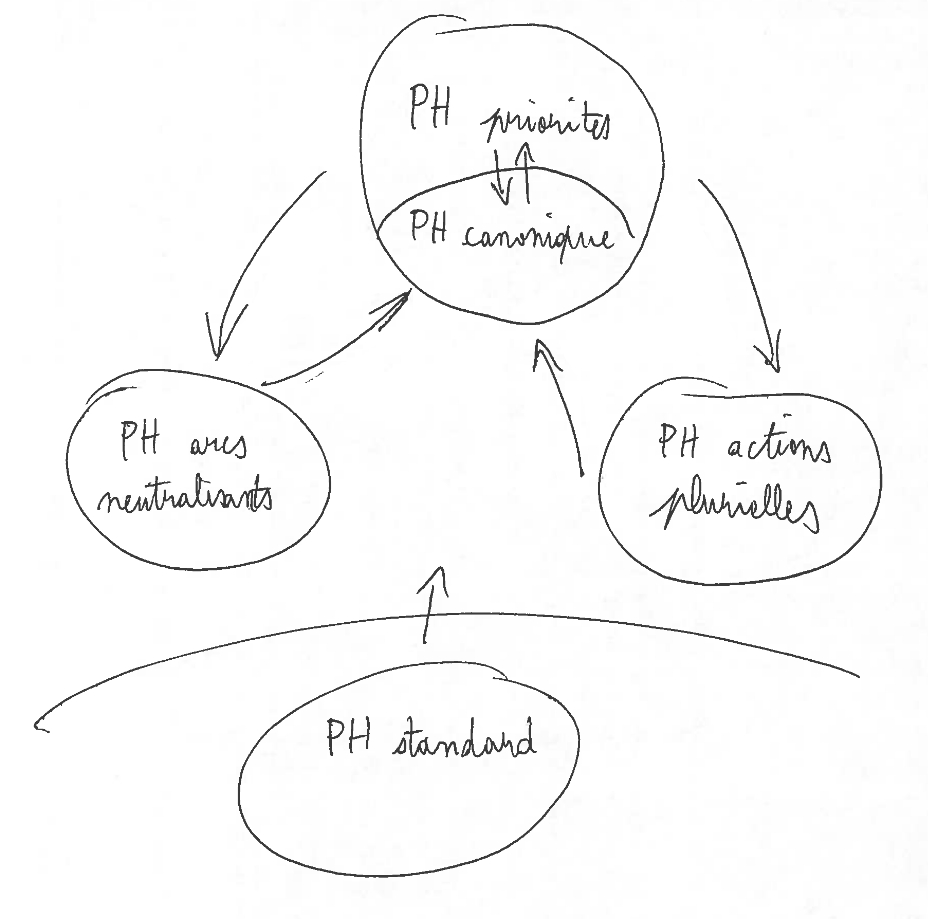
\includegraphics[height=.5\textheight]{figs/PH1.png}
\end{center}

Toutes les sémantiques développées sont équivalentes
\begin{itemize}
  \item Importantes possibilités d'expression
  \item Liens avec d'autres formalismes
  \item Au prix d'une complexité parfois exponentielle
  \item Forme canonique
\end{itemize}

\end{frame}



\begin{frame}[c]
  \frametitle{Traductions depuis et vers d'autres modèles discrets}

\begin{center}
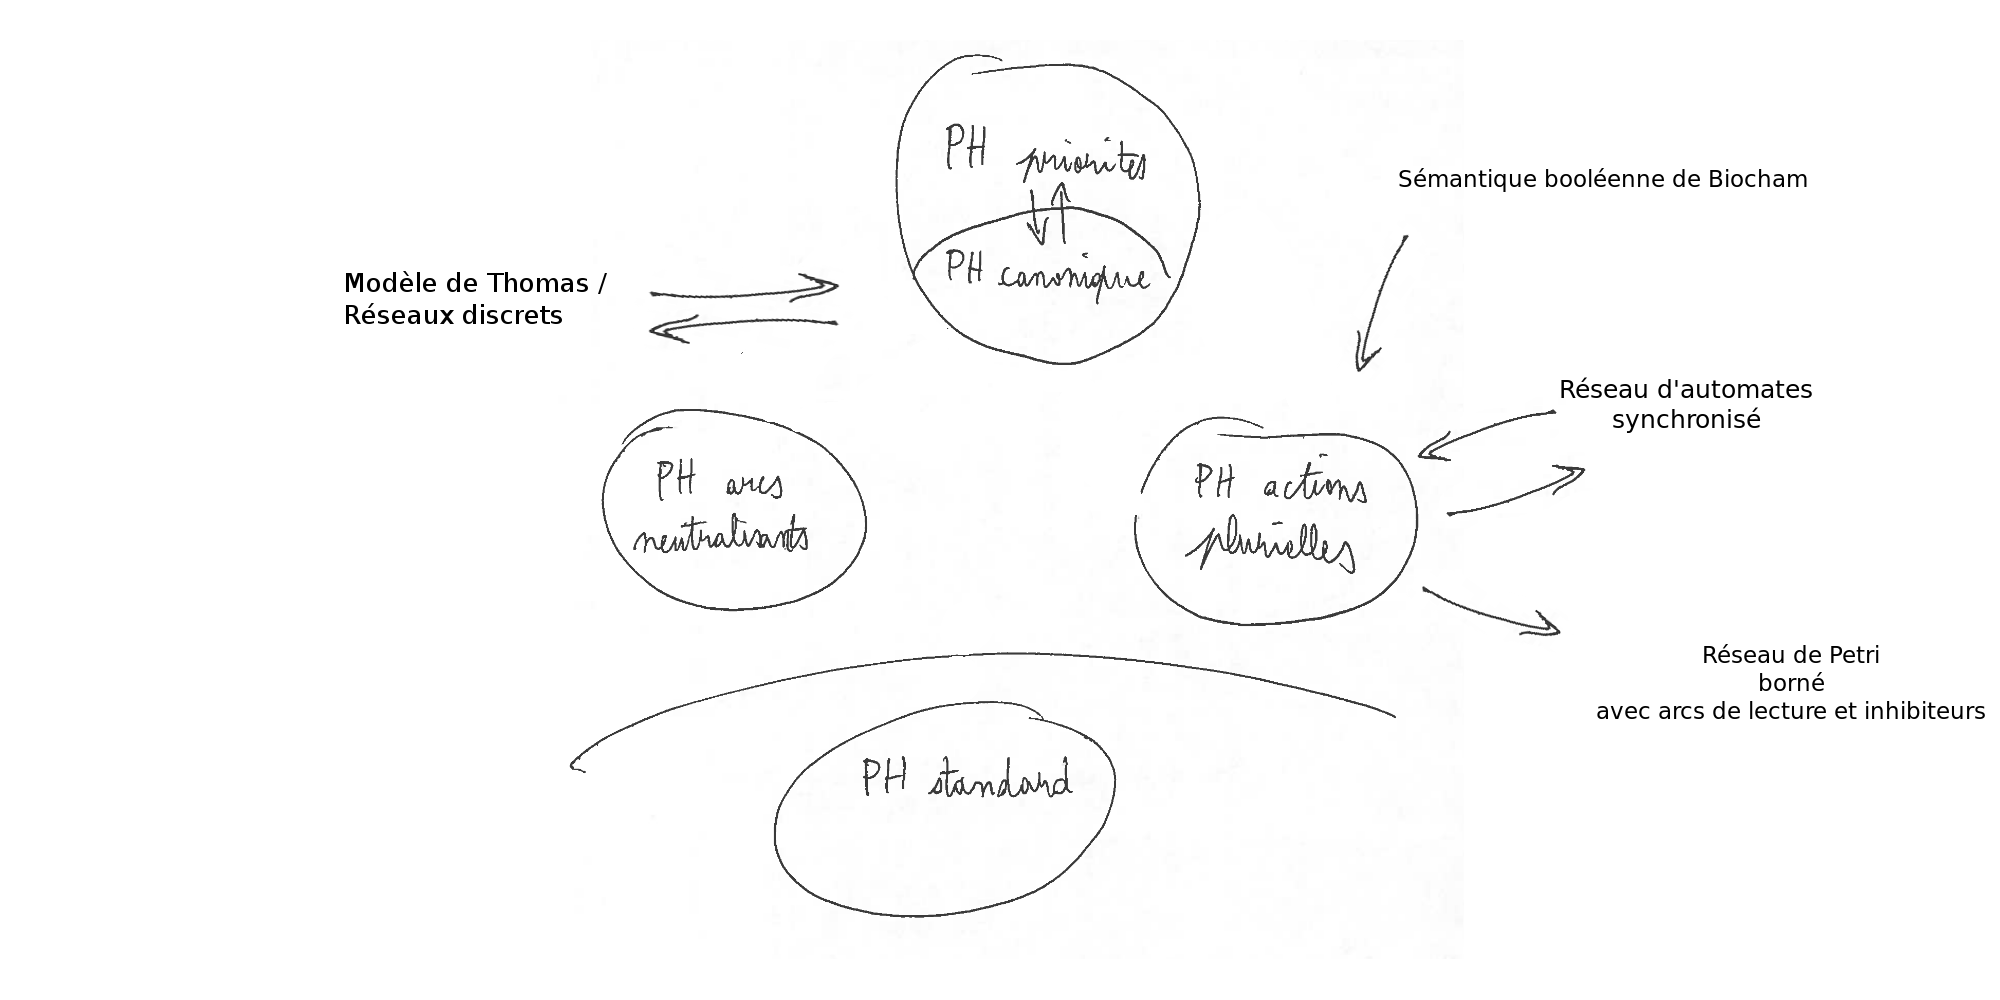
\includegraphics[height=.5\textheight]{figs/PH2.png}
\end{center}

\begin{itemize}
  \item Équivalence avec les réseaux discrets / le modèle de Thomas
  \item Équivalence avec les réseaux d'automates synchronisés
  \item Traduction vers les réseaux de Petri avec arcs inhibiteurs (+ bornitude)
  \item Traduction depuis la sémantique booléenne de Biocham.
\end{itemize}

\end{frame}
